\subsubsection{Attribute Based Access Control} \label{ABAC_SOTA}

\acrfull{abac} is an automated access control model by NIST\footnote{\url{https://csrc.nist.gov/projects/abac/}, accessed 01 April 2019}. In its core it is based on automatic execution of granting and denying the access depending on attributes and policies. \acrshort{rbac} can be also referred to as Policy (\acrshort{pbac}) or Claims (\acrshort{cbac}) Based Access Control\footnote{\url{https://www.hpl.hp.com/techreports/2009/HPL-2009-30.pdf}, accessed 01 April 2019}. XACML standards is based on \acrshort{abac} and is explained in Section \ref{sec:xacml}. It is often denoted as the evolution of \acrshort{rbac}. This model can implement \acrshort{mac} and \acrshort{dac} models as well.

In \acrshort{abac}, access is assigned based on attributes and characteristics of the user – subject which is making the request, environment conditions and information asset – resource object that is requested. With the help of these attributes, granular policies for granting and denying access can then be established. Every policy combines a set of attributes and is executed by the Boolean logic, e.g. IF the requestor is an accountant, THEN allow read access to contracts.

\begin{figure}[ht]
    \centering
    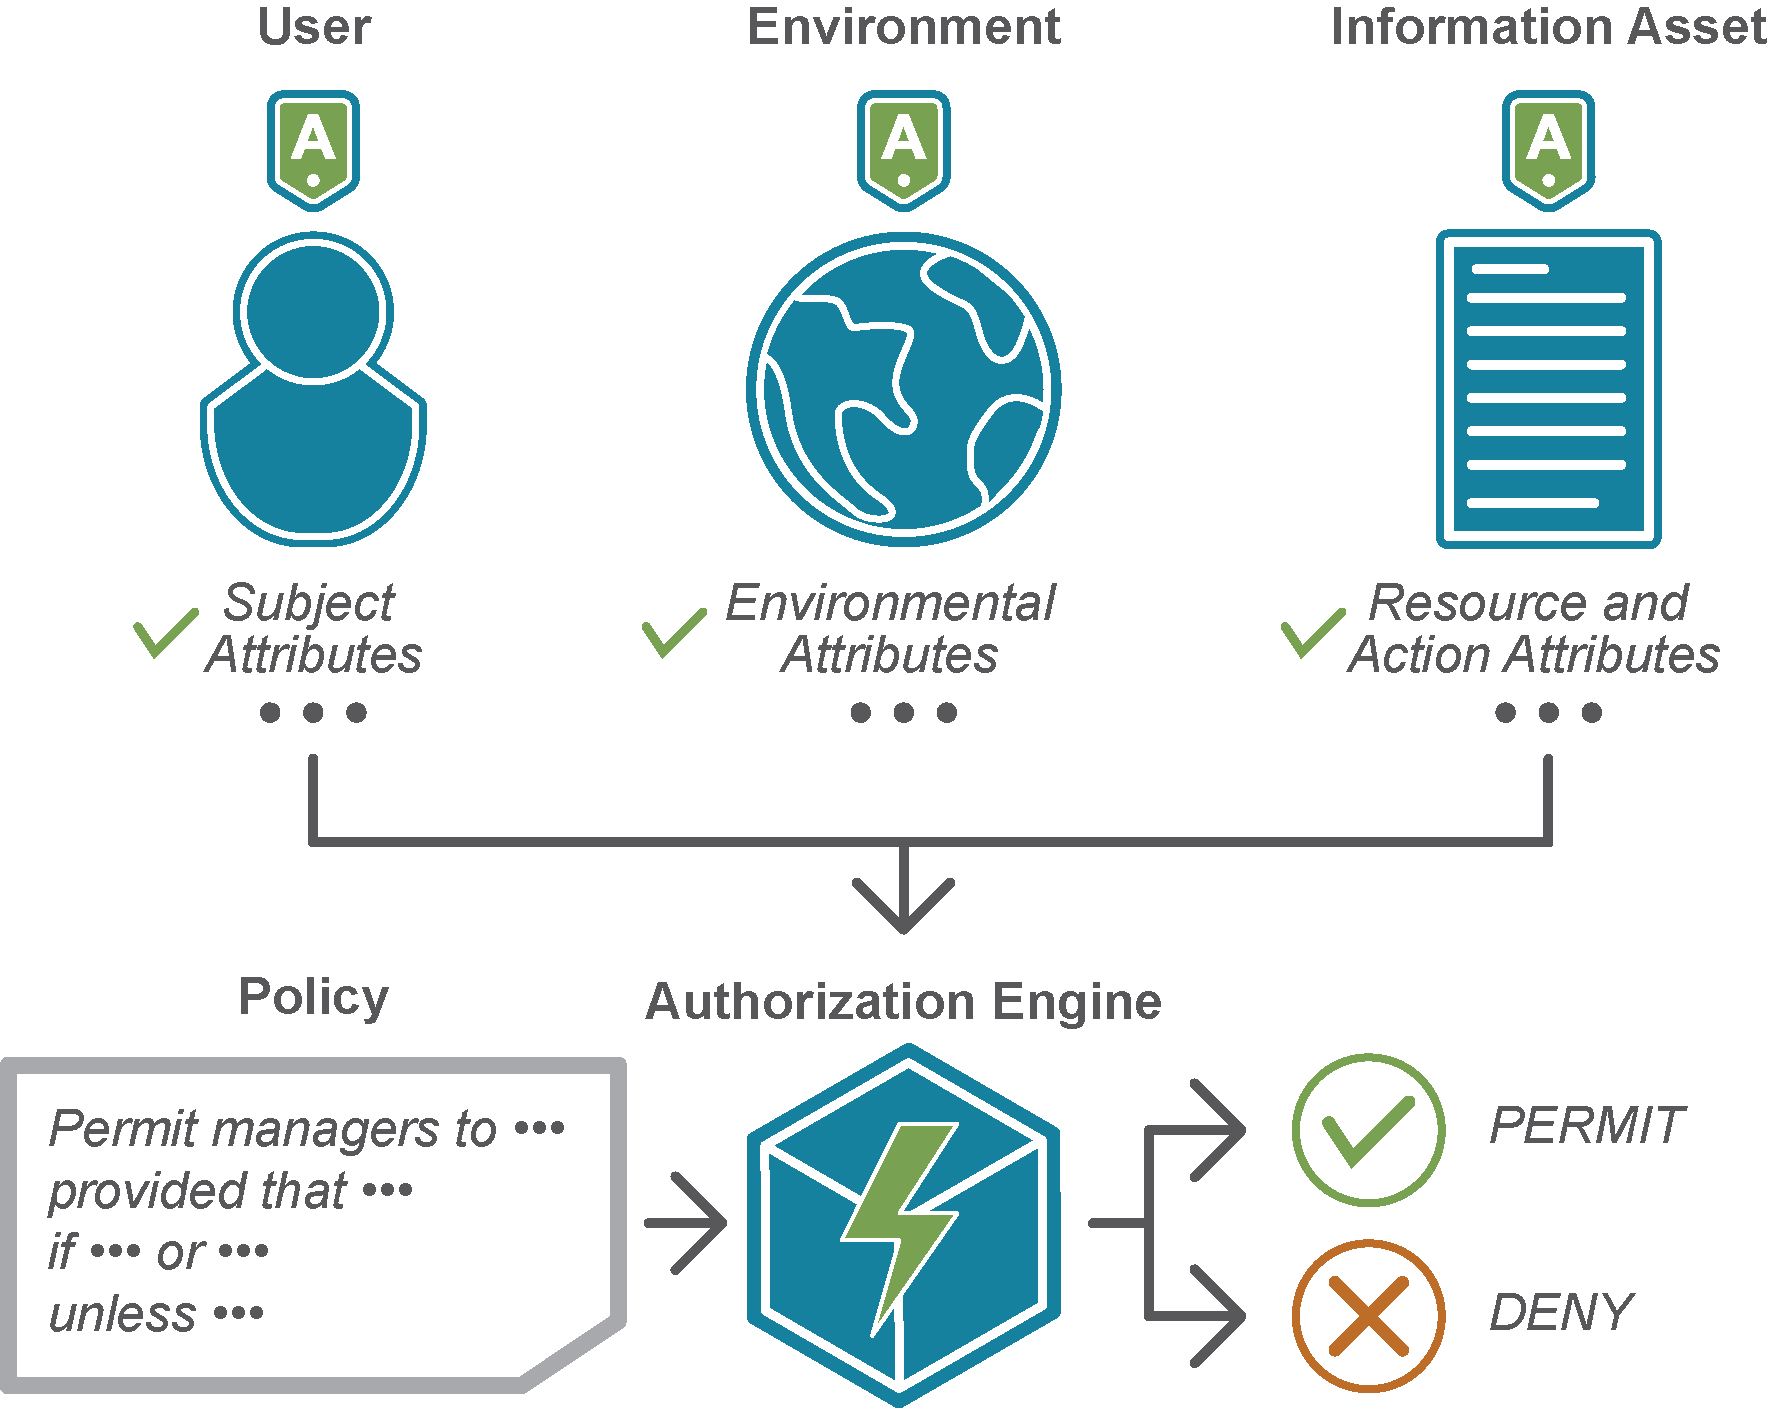
\includegraphics[width=.7\textwidth]{ABAC}
    \caption{Explanation! + SOURCE: https://www.axiomatics.com/attribute-based-access-control/}
    \label{fig:ABAC_diagram_sota}
\end{figure}